\documentclass[10pt]{article}
\usepackage[usenames]{color} %used for font color
\usepackage{amssymb} %maths
\usepackage{amsmath} %maths
\usepackage[utf8]{inputenc} %useful to type directly diacritic characters
\usepackage{tikz}
\usetikzlibrary{automata,positioning}
\begin{document}
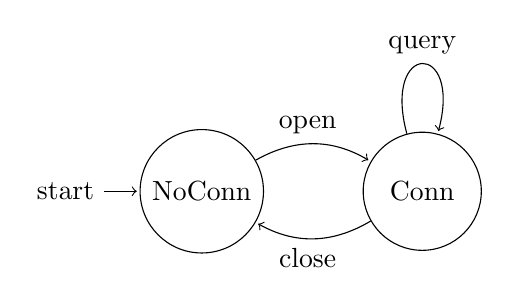
\begin{tikzpicture}[shorten >=1pt,node distance=2.8cm,on grid,auto] 
   \node[state,initial] (q_0)   {NoConn}; 
   \node[state] (q_1) [right=of q_0, minimum size=1.5cm] {Conn}; 
    \path[->] 
    (q_0) edge [bend left] node[pos=0.45] {open} (q_1) 
    (q_1) edge [loop above] node {query} (q_1) 
          edge [bend left] node[pos=0.55] {close} (q_0) ;
\end{tikzpicture}

\end{document}